\newpage
\section{Extension de l’application}
\subsection{Structure d'un fichier grilleXX.txt}
Ce fichier commence  par les dimensions de la futur grille, d’abord le nombre de région par 
largeur, puis un espace, ensuite le nombre de région par hauteur, puis un saut de ligne.
Le fichier continue par les valeurs des cases fixes espacées d’un espace entre chaque valeur. 
Les cases modifiables sont représentées par un zéro. Chaque ligne du fichier représente une 
ligne du sudoku comme suit la figure ci-dessous.
\begin{figure}[ht]
  \caption{\label{annexe1} fichier text}
  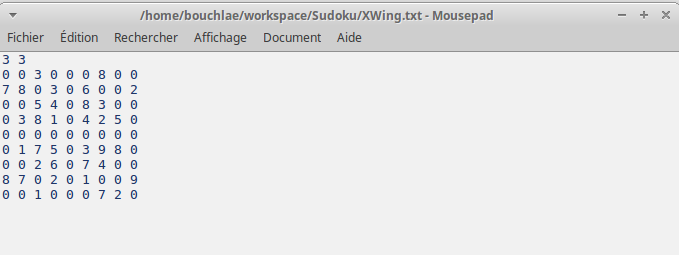
\includegraphics [width=80mm]{images/Fichier_text.png} \\[0.5cm]
\end{figure}

Le modèle transforme le fichier texte figure6 en cette grille figure7\\

\begin{figure}[ht]
  \caption{\label{annexe1} grille modélisé}
  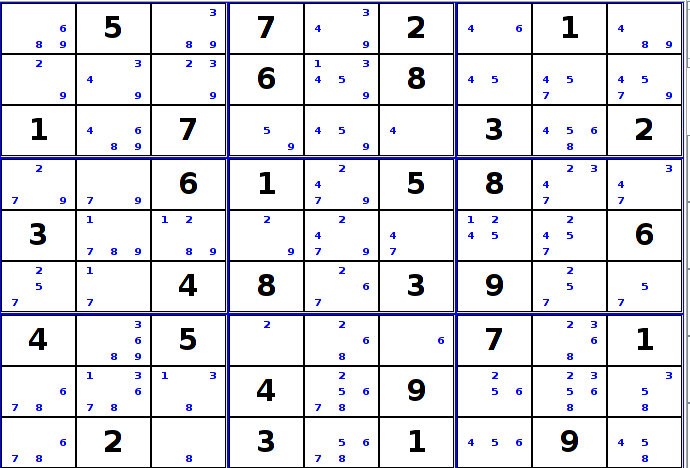
\includegraphics [width=80mm]{images/fichier_type.png} \\[0.5cm]
\end{figure}
\newpage
\subsection{Création d’une règle}
On peut ajouter de nouvelle règle à l’application, pour celà il faut générer un rapport, 
c’est-à-dire être une sous-classe de ReportGenerator.\\
Une règle est constituée de sa description, d’une liste de valeur (ajout d’une valeur dans 
une case ou suppressions des candidats dans une ou plusieurs case(s) ) et de quatre ensembles 
(pour la surbrillance de l’aide) : 
\begin{itemize}
\item DELETION\_CELLS (rouge foncé): ensemble des cellules concernées par la suppression d’un candidat
\item DELETION\_UNITS (rouge clair): les unités des cellules de l'ensemble précédent
\item DECISIVE\_CELLS (bleu foncé): ensemble des cellules qui se base sur le raisonnement de la règle
\item DECISIVE\_UNITS (bleu clair): les unités des cellules de l'ensemble précédent
\end{itemize}
Si DELETION\_CELLS n’est pas vide on peut en conclure que l’action de la règle est de supprimer 
les candidats de la liste dans cet ensemble de cellules. Au contraire si cet ensemble est vide 
c’est qu’on doit ajouter la valeur  dans DECISIVE\_CELLS.\\
Si la règle n’aboutit à aucune avancée dans la grille (suppression candidat ou ajout valeur) 
elle renvoit null.


\newpage
\section{Interface}

Notre application se présente de la manière suivante :\\
une barre de menu située au nord de la fenêtre vous permettra de choisir 
une action à réaliser parmi toutes les fonctionnalités qui vous sont proposées.\\
\\
La grille de sudoku occupe le centre de notre application et se retrouve accompagnée 
d'une colonne, à l'est de la fenêtre, vous permettant de sélectionner 
parmi des boutons raccourcis, les fonctionnalités les plus utilisées telle défaire, 
refaire une action, demander un indice, réinitialiser la grille etc, puis, 
une zone d'aide, située en bas de la grille.\\

Il vous est également possible d'utiliser votre clavier afin de profiter 
des fonctionnalités que vous offre notre application.\\
Pour ce faire, il vous suffit de saisir la combinaison appropriée, combinaison 
que vous pourrez retrouver en consultant les listes des fonctionnalités disponibles dans le menu, 
au nord de l'application, où coïncide chaque fonctionnalité avec sa combinaison 
de la forme CTRL+LETTRE, qu'il vous suffit d'utiliser en appuyant simultanément 
sur la touche contrôle et la lettre correspondante à l'action souhaîtée. \\

Pour ajouter/retirer des possibilités dans la grille, il vous suffit d'utiliser 
le bouton droit de la souris tandis que pour ajouter/retirer des candidats, il 
faudra utiliser le bouton gauche de votre souris.

\subsection{Le composant principal - La grille}

La grille est constituée de deux classes : Grid et Cell.
Ces deux classes héritent de JPanel, conteneurs simples.

\paragraph{Cell}
    
La classe Cell est chargée d'afficher une cellule et possède donc un CellModel.
Une Cell est constituée de plusieurs JPanel disposés sur un CardLayout (layout
permettant de n'afficher qu'un seul composant à la fois). Ces JPanel sont
destinés à accueillir des symboles (ici des JLabel) représentant chaque valeur
possible, à l'exception du premier qui correspond à une cellulesans valeur.
Ce premier JPanel contient donc d'autres JPanel, disposés sur un GridLayout
(layout permettant de répartir les composant sur une grille occupant tout l'espace),
chargés d'afficher les candidats.

Une Cell dispose d'une bordure pour bien la délimiter.
Le GridLayout associé aux candidats est configuré pour les placer dans une grille
carré de côté n = partie entière supérieur de la racine carré du nombre de valeur
possible. En pratique, si les dernières lignes sont vides, la grille ne sera pas
carrée (ex: sudoku 6x6 -> candidats répartits sur une grille 2x3 au lieu de 3x3).

En ce qui concerne les controlleurs, une Cell écoute les changements sur les
propriétés liées à son modèle : VALUE pour afficher la bonne valeur (ou les
candidats s'il n'y a pas de valeur), et CANDIDATE pour afficher, ou non, chaque
candidat.

L'effet de changement de couleur de fond lors du survol à la souris est produit
en écoutant les évènements d'entrée et de sortie du composant liés à la souris,
et ça pour chaque JPanel contenant un symbole (valeur ou candidat). Le traitement
effectué est un simple affichage, ou non, du fond du JPanel, initialisé avec une
couleur semi-transparente, pour laisser transparaitre le fond de Cell (qui est
un JPanel).

Tous ces controlleurs sont assez directs. En revanche, le clique souris ne
modifie pas directement le modèle. En effet, il nous était impossible de modifié
directement le modèle étant donné que nous devions faire passer toutes les actions
par l'historique. Nous avons donc choisi de lancer un évènement de changement de
propriété (VALUE ou CANDIDATE selon le clique et le composant) à destination
principalement de Grid qui, lui possède tous les composant du modèle nécessaires.

\paragraph{Grid}
    
La classe Grid est chargée d'afficher une représentation d'un SudokuModel.
L'affichage des cellules est délégué à un groupe de Cell qui sont regroupées en
régions. C'est aussi cette classe qui s'occupe de récupérer les évènements de
clique souris depuis les Cell et, ainsi, crée les Command correspondantes et les
envoie dans l'historique.

La disposition des cellules se fait gràce à un GridLayout contenant des JPanel
(représentant les régions) disposant d'une bordure. Ces JPanel composés eux-mêmes
de Cell dans des GridLayout.

En ce qui concerne l'aide, cette classe écoute les changement de la propriété liée
LAST\_REPORT de RuleManager (l'écouteur est envoyé au RuleManager du modèle (SudokuModel)
par l'intermédiaire de ce dernier. Lorsque cette propriété change, la couleur de fond
des cellules sont mise à jour. Si la nouvelle valeur de la propriété ne vaut pas null,
les cellules correspondant aux coordonnées dans les ensembles du Report voient leurs
couleur de fond changer au profit de celle contenue dans le nom de son ensemble
(CellSetName). Si la nouvelle valeur est null, alors les cellules liées à l'ancien
Report reprennent leur couleur de fond initiale.

Le changement de grille est assez particulier puisque le chargement d'une sauvegarde
implique seulement de changer un attribut (GridModel) dans le modèle tandis que 
le chargement d'une nouvelle grille implique de changer la référence du modèle
(puisqu'on en crée un nouveau). Aussi, la grille chargée, nouvelle ou sauvegardée,
peut être de dimension différente de la précédente.

Pour régler le premier problème, Grid écoute tout changement de grille de son
SudokuModel (propriété GRID) et utilise la méthode setModel() sur ce dernier
(qui est le même objet) ainsi la méthode setModel() est appelée dans les deux cas.

Le deuxième problème est réglé dans la méthode setModel(). Si l'ancienne grille
et la nouvelle sont de même taille, alors le modèle de chaque Cell est mis à jour.
Sinon, tous les composant graphiques interne de Grid sont retirés et on recommence
le procéssus de construction à partir de la création de la vue (createView())


\begin{figure}[ht]
  \caption{\label{annexe6} interface sudoku}
  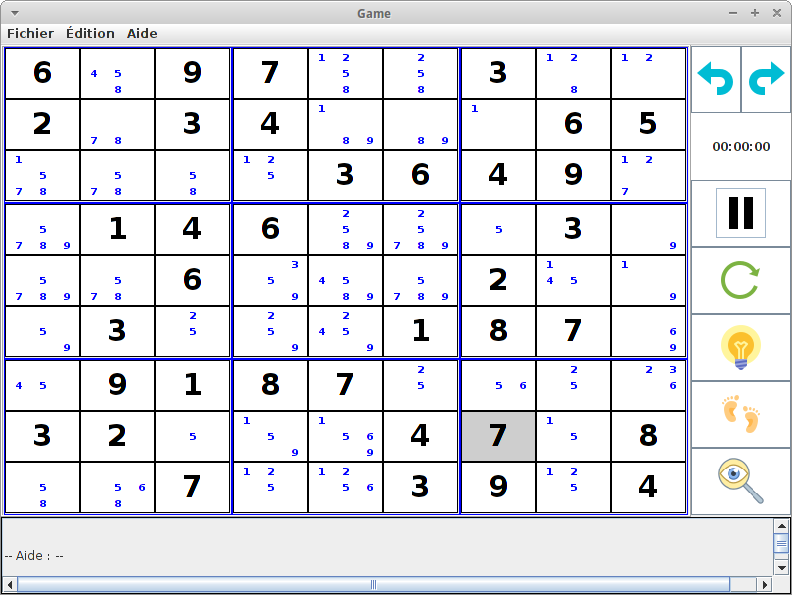
\includegraphics [width=130mm]{images/interface.png} \\[0.5cm]
\end{figure}

\newpage
\section{Jouabilité}
Dans le menu fichier, vous pourrez choisir entre choisir 
une nouvelle grille (par défault, la grille numéro 2 est choisie),
ouvrir un fichier de sauvegarde, 
sauvegarder la partie ou encore quitter la partie.

\begin{figure}[ht]
  \caption{\label{annexe7} menu fichier}
  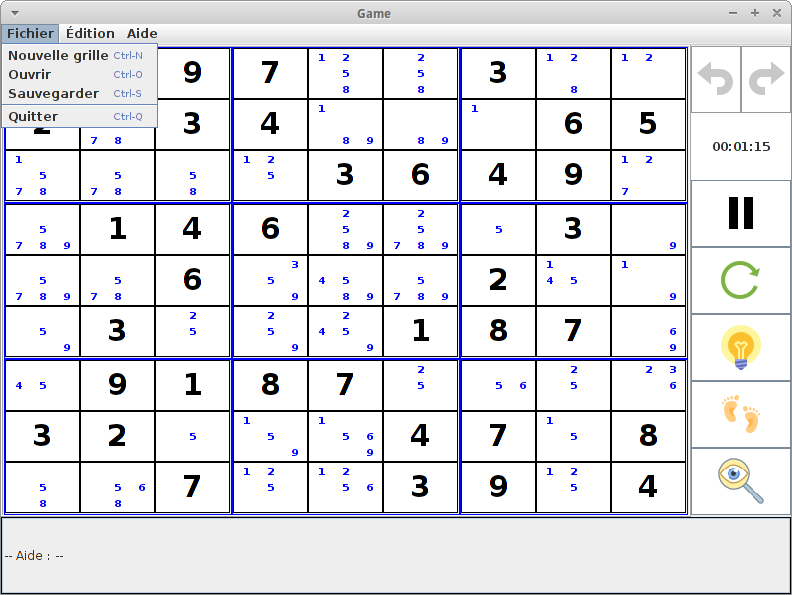
\includegraphics [width=130mm]{images/fichier.png} \\[0.5cm]
\end{figure}

\newpage
Dans le menu édition, vous aurez la possibilité de réinitialiser la grille, 
c'est-à-dire remettre votre grille choisie dans son état initial, 
résoudre pas à pas qui consiste à remplir les cases vides de la grille
en expliquant comment procéder grâce à un petit texte apparaissant en bas de l'écran, 
l'indice, donne un message d'aide et surligne la ligne correspondant d'une couleur bleu 
sans donner la réponse, demander la solution complète de la grille, 
refaire l'action et défaire l'action précédente.

\begin{figure}[ht]
  \caption{\label{annexe8} menu édition}
  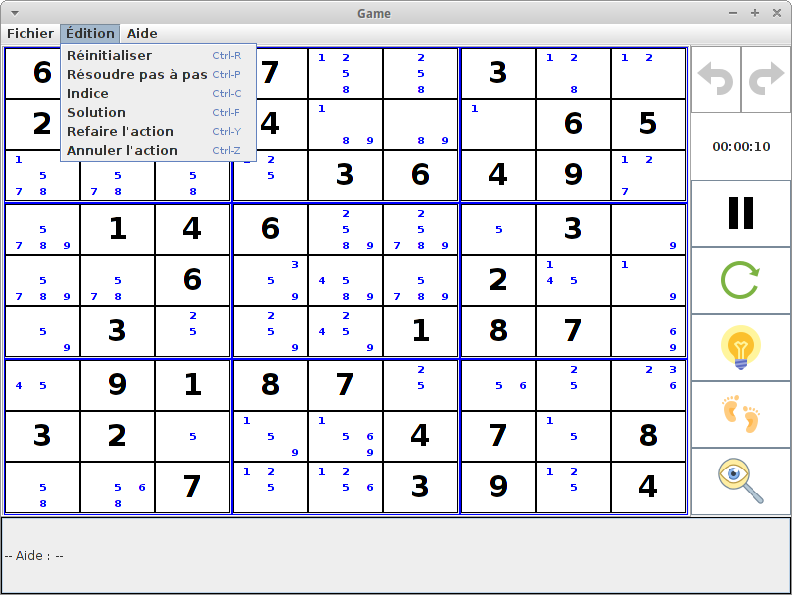
\includegraphics [width=130mm]{images/edition.png} \\[0.5cm]
\end{figure}

\newpage
Dans le menu aide, vous aurez la possibilité de consulter 
les règles du jeu et un guide d'utilisation de notre application.

\begin{figure}[ht]
  \caption{\label{annexe9} menu aide}
  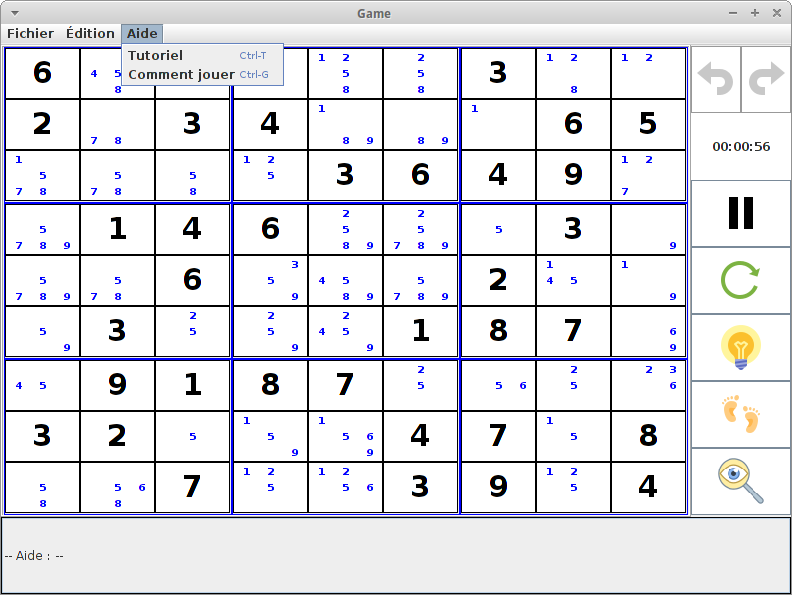
\includegraphics [width=130mm]{images/aide.png} \\[0.5cm]
\end{figure}

\newpage
Toutes ces opérations sont également accessibles grâce aux raccourcis clavier suivant :
\begin{itemize}
 \item CTRL+N : nouvelle grille
 \item CTRL+O : ouvrir un fichier de sauvegarde
 \item CTRL+S : sauvegarder sa partie
 \item CTRL+Q : quitter le jeu
 \item CTRL+R : réinitialiser
 \item CTRL+P : résoudre pas à pas
 \item CTRL+C : avoir un indice
 \item CTRL+F : solution complète
 \item CTRL+Y : refaire l'action
 \item CTRL+Z : annuler l'action
 \item CTRL+T : tutoriel
 \item CTRL+G : comment jouer
\end{itemize}

\newpage
Lorsque vous appuyez sur le bouton pause, une fenêtre apparaît 
et vous propose de reprendre la partie ou de la quitter.
\begin{figure}[ht]
  \caption{\label{annexe10} pause}
  
\includegraphics [width=70mm]{images/pause.png} \\[0.5cm]
\end{figure}

\newpage
Si vous appuyez sur le bouton solution, la grille sera remplie entièrement.
\begin{figure}[ht]
  \caption{\label{annexe11} solution complète}
  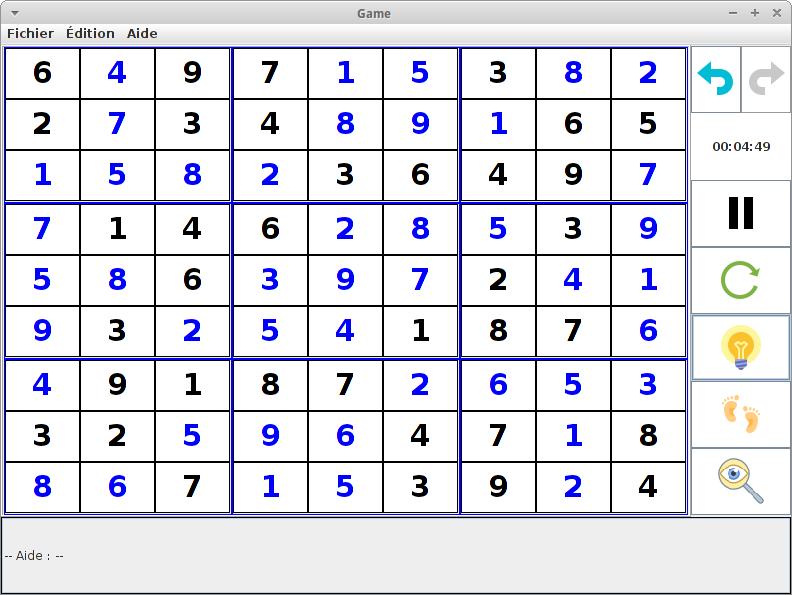
\includegraphics [width=130mm]{images/solution.png} \\[0.5cm]
\end{figure}

\newpage
Vous avez la possibilité de réinitialiser la grille de sudoku 
et ainsi de recommencer la partie. 
\begin{figure}[ht]
  \caption{\label{annexe12} réinitialisation}
  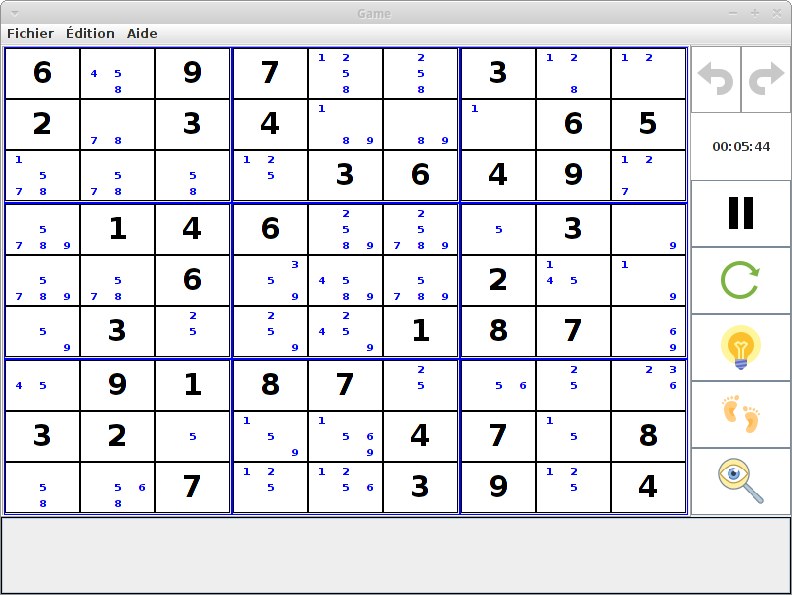
\includegraphics [width=130mm]{images/reinit.png} \\[0.5cm]
\end{figure}

\newpage
Si vous demandez un indice, vous pourrez avoir un texte d'aide 
et pourrez compléter la grille en vous aidant de la surbrillance 
des cases concernées.  
\begin{figure}[ht]
  \caption{\label{annexe13} indice}
  
\includegraphics [width=130mm]{images/clue.png} \\[0.5cm]
\end{figure}

\newpage
En choisissant la méthode pas à pas, vous bénéficierez à la fois de conseils
pour remplir la grille mais également de la réponse de la case concernée 
vous permettant de résoudre la grille de sudoku. 
\begin{figure}[ht]
  \caption{\label{annexe14} pas à pas}
  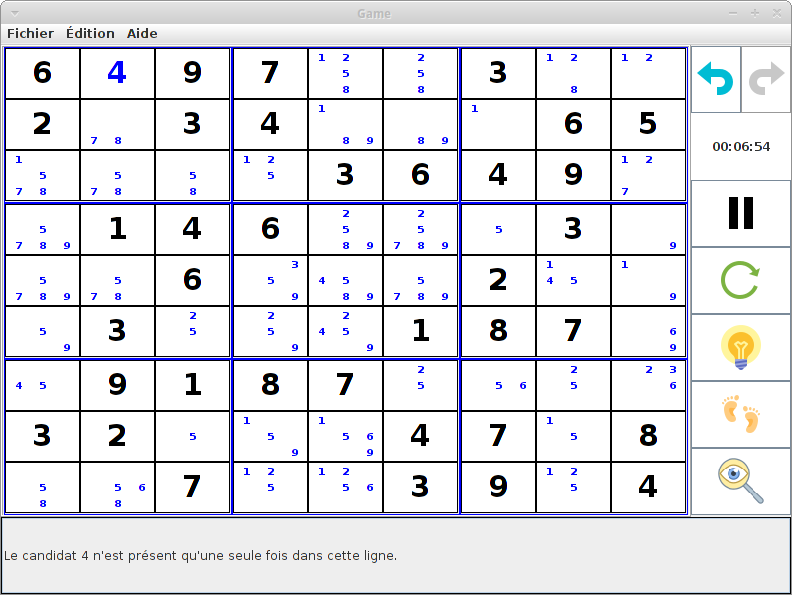
\includegraphics [width=130mm]{images/pas.png} \\[0.5cm]
\end{figure}

\newpage
Il vous est posssible de demander une nouvelle grille, en chargeant 
un fichier grilleXX.txt. L'application supporte différents formats de grilles. 
\begin{figure}[ht]
  \caption{\label{annexe15} nouvelle grille}
  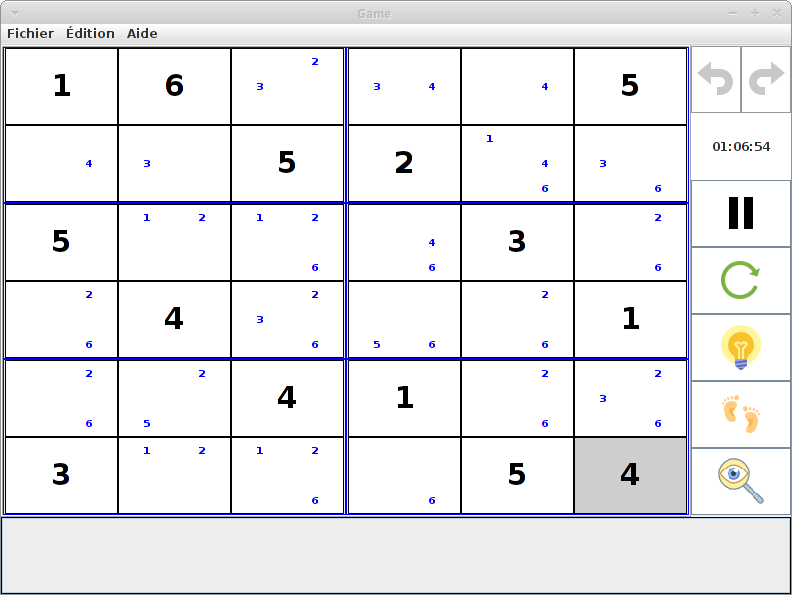
\includegraphics [width=130mm]{images/newGrid.png} \\[0.5cm]
\end{figure}

\newpage
\section{Difficultés rencontrées}
Lors de la conception de notre projet, nous avons rencontrés quelques difficultés :
\begin{itemize}
 \item gestion du temps, où chaque semaine, nous nous fixions des objectifs à atteindre,
 \item utilisation et prise en main du logiciel git et du site 
	    \href{https://github.com/yuki1996/Sudoku}{github.com}, 
 \item respect des demandes de la part du client, 
 \item incompatibilité/réajustement lors de réunion de différents travaux des membres du groupe
 \item essais infructueux, sur deux semaines, d'une implantation de la partie vue
    de la grille avec des JTable. Certains fichiers sont encore dans le projet (sudoku.view.test\_jtable)
    mais inutilisés.
\end{itemize}
\section{Répartition du travail}
Dans un premier temps, nous avons tous ensemble commencer à réfléchir à l'architecture du modèle.
Puis au moment où nous avons eu une structure claire, Loïc, Paul et Laëtitia ont codé le modèle quant
à Florian, il a commencé à concevoir et élaborer le design et les fonctionnements de l'application du jeu.
Quant le modèle fut fini et la réflexion sur les structures des règles et du gestionnaire d'heuristiques
achevée Laëtitia et Paul se sont mis à les coder, y compris l'historique. Quant à Loïc, il est parti avec 
Florian sur la partie graphique du projet mais plus centré sur les composants grille et cellule (surbrillance...)
Pour finir, chacun a donné un coup de main dans toutes les parties du projet pour régler les derniers beugs et erreurs.

\newpage
\section{Conclusion}
Ce projet nous a apporté une grande expérience car il s'agit 
de notre premier ``gros'' projet en équipe de plus de deux personnes.

Afin de réaliser un travail commun, nous avons opté pour un service 
de gestion de développement de logiciels, utilisant le logiciel 
de gestion de versions Git ainsi que le service web d'hébergement \url{https://github.com/}.

Ce dernier fut, pour nous, d'une grande aide, ce fut une toute nouvelle façon de 
procéder que nous a donné comme opportunité ce projet même si la prise en main 
fut assez compliquée.

Pour finir, ce projet fut, pour nous, très enrichissant car il nous a permi de réunir
l'ensemble de nos connaissances au sein d'un même projet. Nous avons fait le choix 
de développer notre application dans le langage de programmation Java, qui est un langage
très intéressant pour le développement d'applications graphiques.

\begin{thebibliography}{9}
 \bibitem{Site Internet}
          \url{https://www.mots-croises.ch/Sudoku.htm}
 \bibitem{Site Internet}
          \url{http://www.le-sudoku.fr/}
\end{thebibliography}

\subsection*{Logiciels utilisés}
\begin{itemize}
\item Eclipse (Java)
\item ObjectAid (plugin Eclipse pour creer les diagrammes de classes)
\item Git
\item Kile (LaTex)
\end{itemize}

\section{Annexes}
\begin{figure}[ht]
  \caption{\label{annexe16} Diagramme model}
  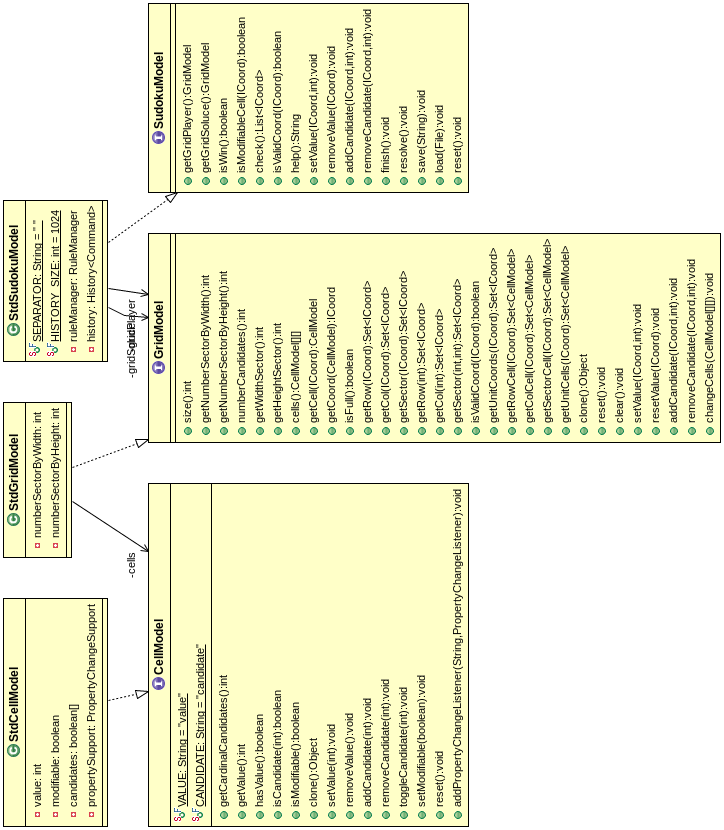
\includegraphics [width=160mm]{images/model.png} \\[0.5cm]
\end{figure}

\begin{figure}[ht]
  \caption{\label{annexe17} Diagramme history}
  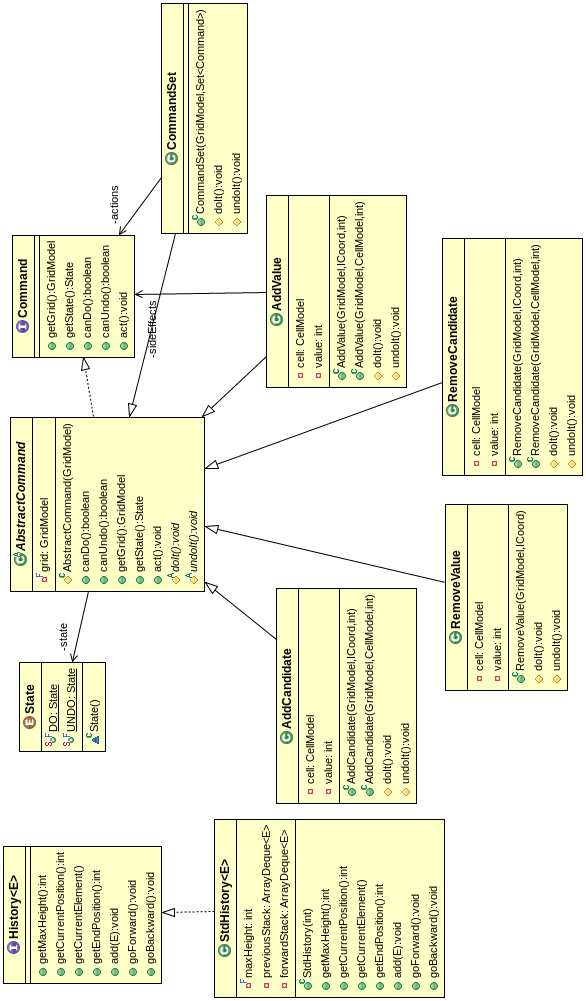
\includegraphics [width=140mm]{images/history.png} \\[0.5cm]
\end{figure}

\begin{figure}[ht]
  \caption{\label{annexe18} Diagramme heuristic}
  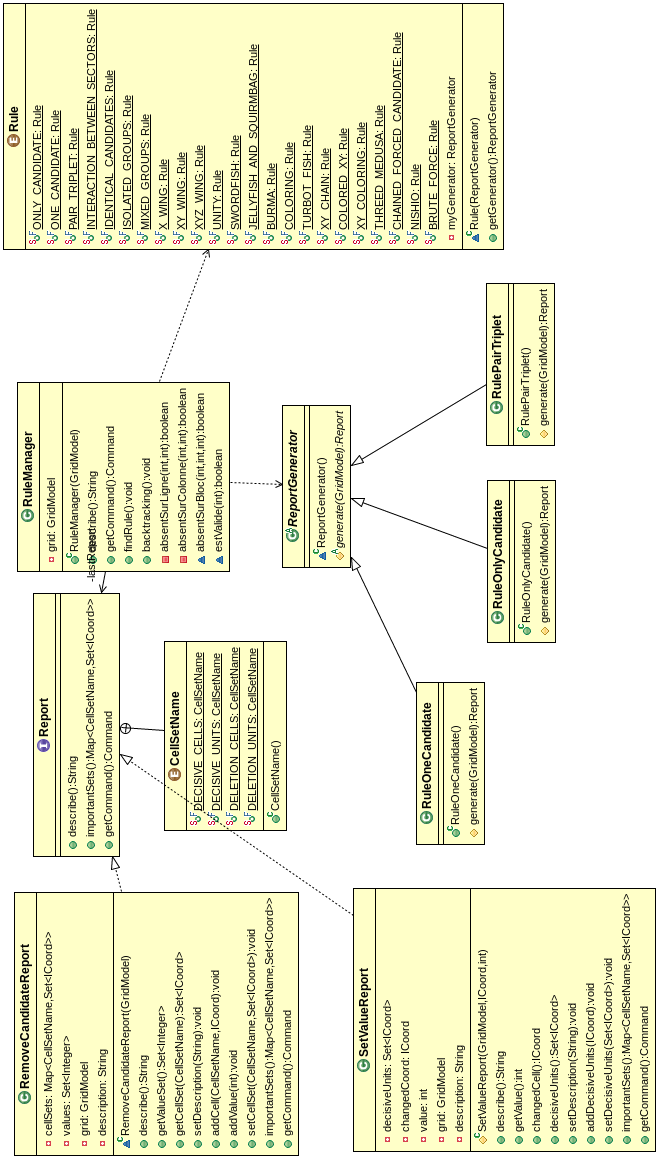
\includegraphics [width=140mm]{images/heuristic.png} \\[0.5cm]
\end{figure}



